% Combined slides for the merged self-study (harness architecture plus
% open-source model support). Build with tools/build_slides.sh <study-dir>.
% Citations come from report/refs.bib via BIBINPUTS set by build_slides.sh.
% One message per frame; every number matches report/main.tex.
\documentclass[aspectratio=169,11pt]{beamer}

\usetheme{Madrid}
\usecolortheme{default}
\setbeamertemplate{navigation symbols}{}
\usepackage[T1]{fontenc}
\usepackage{amsmath,amssymb}
\usepackage{booktabs}
\usepackage{array}
\usepackage{graphicx}
\usepackage[table]{xcolor}
\usepackage{tikz}
\usetikzlibrary{positioning,arrows.meta}
\usepackage[numbers]{natbib}
\usepackage{hyperref}

\definecolor{nativecol}{HTML}{0072B2}
\definecolor{genericcol}{HTML}{009E73}
\definecolor{partcol}{HTML}{E69F00}
\definecolor{unattcol}{HTML}{D55E00}
\setbeamercolor{structure}{fg=nativecol}
\setbeamerfont{caption}{size=\scriptsize}

\newcolumntype{L}[1]{>{\raggedright\arraybackslash}p{#1}}

\newcommand{\codex}[0]{Codex}
\newcommand{\occ}[0]{OpenCode}
\newcommand{\ccc}[0]{Claude Code}

% Parametric TikZ styles must live in the preamble: beamer re-tokenizes
% frame content and rejects style definitions with parameters inside frames.
\tikzset{
  ag/.style={draw=#1, line width=0.9pt, rounded corners=1pt, fill=#1!12,
    text=black, minimum width=3.0cm, minimum height=1.05cm, align=center},
  box/.style={draw=black!70, rounded corners=1pt, align=center,
    minimum width=3.6cm, minimum height=0.85cm, inner sep=2pt,
    fill=blue!5, text=black},
  loopdim/.style={box, fill=orange!18},
  conn/.style={draw=black!40, line width=0.35pt},
  proto/.style={draw=black!70, line width=0.7pt, rounded corners=1pt,
    fill=black!5, align=center, minimum width=3.85cm, minimum height=0.95cm,
    inner sep=2.5pt, text=black},
  reqlab/.style={draw=black!40, line width=0.5pt, rounded corners=1pt,
    align=center, minimum width=3.85cm, minimum height=0.85cm,
    inner sep=2.5pt, text=black},
  chip/.style={rounded corners=1pt, align=center, minimum width=3.85cm,
    minimum height=0.85cm, inner sep=2.5pt, text=black},
  rowhead/.style={draw=black!50, line width=0.5pt, rounded corners=1pt,
    fill=black!5, align=center, minimum width=2.3cm, inner sep=2.5pt,
    text=black},
  arr/.style={-{Stealth[length=1.8mm]}, draw=black!60, line width=0.5pt},
  sv/.style={draw=black!70, line width=0.7pt, rounded corners=1pt,
    fill=black!6, text=black, minimum width=2.7cm, minimum height=1.05cm,
    align=center},
  nat/.style={-{Stealth[length=2.4mm]}, line width=1.1pt, nativecol},
  gen/.style={-{Stealth[length=2.4mm]}, line width=1.1pt, genericcol},
  unv/.style={-{Stealth[length=2mm]}, line width=0.8pt, black!45, loosely dotted}}

\title[Harnesses and open-model support]{How Claude Code, Codex, and
OpenCode Build Their Harnesses, and Meet Open-Source Models}
\subtitle{A static source-trace study at pinned commits}
\author[self-study-with-ai]{self-study-with-ai}
\date{\today}

\begin{document}

\begin{frame}
  \titlepage
  \note{Two parts, one static discipline. Part I: what is inside the
  harness that turns a language model into a coding agent, and how
  differently do the three products answer it? Part II: what happens when
  the model on the other end is open source? Nothing was executed; no API
  was called.}
\end{frame}

\begin{frame}{Outline}
  \tableofcontents
\end{frame}

\section{Motivation}

\begin{frame}{Two questions, one evidence discipline}
  \textbf{Part I question.} How do \ccc{}, \codex{}, and \occ{} implement
  their coding-agent harnesses, and where do they genuinely differ?

  \vspace{0.4em}
  \textbf{Why the harness matters.}
  \begin{itemize}
    \item ReAct: interleaving reasoning and acting beats either alone;
      grounded search cut hallucinated failures from 56\% to 0\% on
      HotpotQA~\citep{yao2023react}.
    \item Toolformer: the interrupt, execute, resume protocol behind every
      tool call, with decoding constrained to stop tool-call
      loops~\citep{schick2023toolformer}.
    \item SWE-agent: an agent-tailored interface raised SWE-bench Lite
      resolution from 11.0\% (shell-only) to 18.0\% with GPT-4 Turbo;
      51.7\% of instances had a failed edit, and edit success dropped from
      90.5\% to 57.2\% after one failure~\citep{yang2024sweagent}.
  \end{itemize}
  \note{Part I gap: we know interface design matters; we do not know how
  the shipping products practitioners use actually build it.}
\end{frame}

\begin{frame}{The Part II question}
  A coding agent with a closed model list is a product; one that can run
  against a local model is a platform.

  \vspace{0.4em}
  \textbf{Three surfaces, held constant while the agent varies:}
  Ollama, LM Studio, and the generic OpenAI-compatible server class
  (llama.cpp reference
  server)~\citep{ollamaCompatDocs,lmstudioApiDocs,llamaCppServerDocs}.

  \vspace{0.4em}
  \textbf{Three sub-questions, answered from static traces:}
  \begin{enumerate}
    \item Through which paths can each agent reach an open-weight model?
    \item What must a server provide before the path is usable?
    \item Where do accounting and tooling degrade around open models?
  \end{enumerate}
  \note{Every claim is a code path, a documentation contract, or a labeled
  gap. Community routers enter only as hedged context.}
\end{frame}

\section{Study design}

\begin{frame}{Three systems, three evidence tiers}
  \begin{columns}[T]
    \column{0.32\textwidth}
      \textbf{\codex{}} (OpenAI, Apache-2.0)\\
      open source, pinned \texttt{af70018}\\
      evidence: \emph{pinned code}
    \column{0.32\textwidth}
      \textbf{\occ{}} (anomalyco, MIT)\\
      open source, pinned \texttt{d545d8f} (\texttt{dev})\\
      evidence: \emph{pinned code}
    \column{0.32\textwidth}
      \textbf{\ccc{}} (Anthropic)\\
      core closed; pinned surface \texttt{c3d2e35}\\
      evidence: \emph{docs snapshots + plugin surface}
  \end{columns}

  \medskip
  \textbf{Evidence discipline.}
  \begin{itemize}
    \item Static source traces only: nothing executed, no API called, no
      server started; checkouts treated as read-only untrusted
      data~\citep{codexRepo,opencodeRepo,claudeCodePluginSurface}.
    \item \ccc{} internals are boundaries, not findings; teardowns and
      routers enter only as hedged
      context~\citep{minusXClaudeCodeTeardown,agiflowClaudeCodeInternals,tenguDecoded,%
      claudeCodeRouterContext}.
  \end{itemize}
\end{frame}

\begin{frame}{Trace experiments and anchors}
  Part I: four frozen extractions (plan EXP-PLAN-2026-08-19-v1), every value
  carrying a file:line or snapshot-line anchor. Part II: 12 anchored notes
  (3 codebase, 8 docs, 1 context), briefing-scoped, not pre-registered.
  \begin{center}
    \small
    \begin{tabular}{llr}
\toprule
Trace & Scope & Anchors re-verified\\
\midrule
E1 & turn loops & 59/59\\
E2 & tool surfaces & 131/131\\
E3 & safety policies & 75/75\\
E4 & compaction parameters & 35/35\\
\midrule
& \textbf{total at the pinned commits} & \textbf{300/300}\\
\bottomrule
    \end{tabular}
  \end{center}
  Validation runs are smoke-test plumbing; the extraction artifacts carry
  the findings. All three HEADs matched the pins at every validation.
\end{frame}

\section{Part I: harness architecture}

\begin{frame}{Eight machinery dimensions}
  \begin{center}
    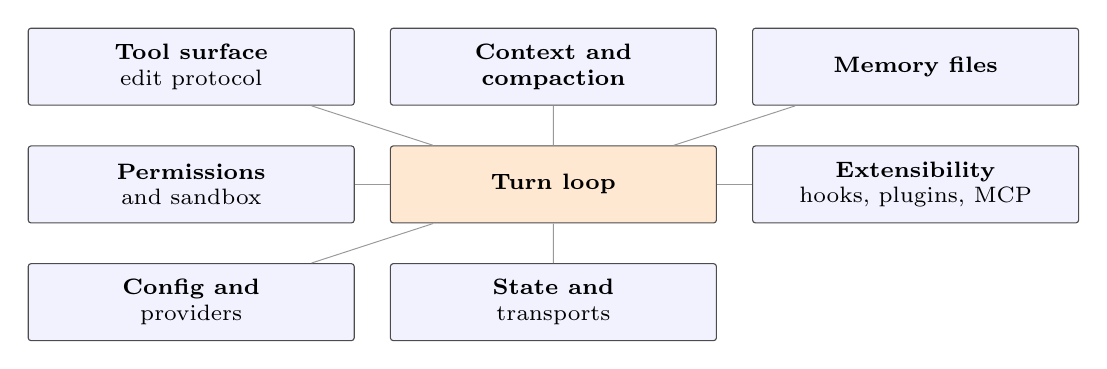
\begin{tikzpicture}[font=\scriptsize, scale=1.15, transform shape]
    \node[loopdim] (loop) at (0,0) {\textbf{Turn loop}};
    \node[box] (tools) at (-4.0, 1.3) {\textbf{Tool surface}\\edit protocol};
    \node[box] (ctx)   at ( 0.0, 1.3) {\textbf{Context and}\\\textbf{compaction}};
    \node[box] (mem)   at ( 4.0, 1.3) {\textbf{Memory files}};
    \node[box] (perm)  at (-4.0, 0) {\textbf{Permissions}\\and sandbox};
    \node[box] (ext)   at ( 4.0, 0) {\textbf{Extensibility}\\hooks, plugins, MCP};
    \node[box] (cfg)   at (-4.0,-1.3) {\textbf{Config and}\\providers};
    \node[box] (state) at ( 0.0,-1.3) {\textbf{State and}\\transports};
    \foreach \n in {tools,ctx,mem,perm,ext,cfg,state}
      \draw[conn] (loop) -- (\n);
    \end{tikzpicture}
  \end{center}
  \vspace{-0.3em}
  Every system implements all eight dimensions; they differ in \emph{how}.
  The abstraction is settled (loop, tools, compaction, permissions,
  extensions); the engineering culture is not (trust boundaries, state
  durability, interface unification). Naming differences (hooks, skills,
  agents) overlay the structural ones rather than masking them.
  \note{The decomposition is grounded in three pinned implementations and
  the framing literature; see the report's summary table for the full
  matrix.}
\end{frame}

\begin{frame}{Turn loops: one contract, three realizations (E1)}
  \small
  \begin{columns}[T]
    \column{0.32\textwidth}
      \textbf{\codex{}: abortable task state machine}
      \begin{itemize}
        \item \texttt{Op} enum, 27 variants; task kinds Regular, Review,
          Compact; preemption via \texttt{Replaced}~\citep{codexRepo}
        \item continue iff \texttt{needs\_follow\_up} = model bit OR
          pending input
        \item steering rejected via an 8-variant taxonomy
      \end{itemize}
    \column{0.32\textwidth}
      \textbf{\occ{}: persistence-driven loop}
      \begin{itemize}
        \item \texttt{while (true)} over persisted message parts; verdict
          compact / stop / continue~\citep{opencodeRepo}
        \item exit re-derived from stored state each iteration
        \item \texttt{doom\_loop} ask after 3 byte-identical calls;
          retry cap 5
      \end{itemize}
    \column{0.32\textwidth}
      \textbf{\ccc{}: closed core, docs-attested seams}
      \begin{itemize}
        \item hook cadences: per session, per turn, per tool
          call~\citep{claudeCodeDocsHooks}
        \item stop-hook override after 8 consecutive blocks
        \item continuation condition, caps, retries undisclosed
      \end{itemize}
  \end{columns}

  \medskip
  Same abstract loop and an explicit anti-loop defense in each system,
  realized three different ways.
\end{frame}

\begin{frame}{Tools and patches: the format converges (E2)}
  \begin{itemize}
    \item \textbf{Registration policy differs.} \codex{}: 32 conditional
      per-turn registrations behind feature and model gates. \occ{}:
      fixed array of 17 tool IDs. \ccc{}: 12 built-ins named in docs plus
      8 more attested by the pinned surface; full registry open~\citep{codexRepo,opencodeRepo,claudeCodeDocsHooks,claudeCodePluginSurface}.
    \item \textbf{The patch format converges across vendors.} \occ{}
      ports the \codex{} \texttt{apply\_patch} grammar near-verbatim
      (``Core types matching the Rust implementation'') and selects it for
      \texttt{gpt-*} model IDs, except \texttt{gpt-4} and
      \texttt{oss}~\citep{opencodeRepo}.
    \item \textbf{Edit robustness is engineered in.} \occ{}'s
      \texttt{edit} runs a 9-stage replacer cascade (similarity 0.65),
      an answer to the fragility SWE-agent measured~\citep{yang2024sweagent}.
    \item \textbf{Negative finding.} \codex{} has no dedicated
      read/glob/grep tools in the extracted registry; the shell carries
      inspection (bounded to the extraction scope).
  \end{itemize}
  \note{The model-ID gate in bullet two is the thread Part II pulls on:
  for open models it decides whether the patch tool exists at all.}
\end{frame}

\begin{frame}{Compaction: literal constants of different kinds (E4)}
  \small
  \begin{columns}[T]
    \column{0.48\textwidth}
      \textbf{\codex{}: fractional trigger}~\citep{codexRepo}
      \begin{itemize}
        \item auto-compact at 9/10 of the resolved window, on a 95\%
          effective window
        \item budgets: 20{,}000 user-message tokens locally; 64{,}000
          retained remotely
        \item rollover compacts mid-turn, then continues
      \end{itemize}
      \smallskip
      \textbf{\occ{}: reserved-buffer trigger}~\citep{opencodeRepo}
      \begin{itemize}
        \item fires at input limit minus min(20{,}000, max-output)
          tokens
        \item pruning-shaped: protects last 40{,}000 tokens of tool
          output; recent messages clamped to 25\% of usable (2{,}000 to
          15{,}000)
      \end{itemize}
    \column{0.48\textwidth}
      \textbf{\ccc{}: seams without numbers}
      \begin{itemize}
        \item \texttt{PreCompact}/\texttt{PostCompact} hooks with manual
          and auto triggers~\citep{claudeCodeDocsHooks}
        \item root CLAUDE.md is re-injected after \texttt{/compact};
          nested files are not~\citep{claudeCodeDocsMemory}
        \item no numeric threshold anywhere in the pinned snapshots
      \end{itemize}
  \end{columns}
\end{frame}

\begin{frame}{Safety: three points on one axis (E3)}
  \footnotesize
  \begin{columns}[T]
    \column{0.32\textwidth}
      \textbf{\codex{}: prevent}
      \begin{itemize}
        \item OS sandbox (Seatbelt, bubblewrap, seccomp) plus Starlark
          rule engine, strictest-wins~\citep{codexRepo,codexDocsSandboxing}
        \item ships no usable policy file; trust-gated project config
      \end{itemize}
    \column{0.32\textwidth}
      \textbf{\occ{}: recover}
      \begin{itemize}
        \item in-process ruleset only; default \texttt{*}:~allow, narrow
          friction at dot-env reads and doom loops~\citep{opencodeRepo}
        \item no OS sandbox in the pinned tree; per-step snapshots with
          revert carry the safety story
      \end{itemize}
    \column{0.32\textwidth}
      \textbf{\ccc{}: layer}
      \begin{itemize}
        \item permission rules before every tool; OS sandbox scoped to
          Bash and its children only~\citep{claudeCodeDocsPermissions,claudeCodeDocsSandboxing}
        \item protected paths deny writes with no per-path exemption;
          enterprise kill switches
      \end{itemize}
  \end{columns}
\end{frame}

\begin{frame}{State and interfaces: convergence in shape, not substrate}
  \begin{itemize}
    \item \textbf{State.} \codex{}: append-only inspectable JSONL plus a
      repairable SQLite mirror; exact replay across compaction. \occ{}:
      event-sourced SQLite plus shadow-git file snapshots at every step.
      \ccc{}: undisclosed; only subagent transcripts documented (30-day
      cleanup default)~\citep{codexRepo,opencodeRepo,claudeCodeDocsSubagents}.
    \item \textbf{Interfaces.} \codex{}: one JSON-RPC protocol behind
      every frontend. \occ{}: local HTTP server consumed by its TUI,
      plus ACP and 38 built-in LSP servers feeding diagnostics back into
      edits. \ccc{}: CLI, IDE, and desktop surfaces attested; transports
      closed~\citep{codexRepo,opencodeRepo,claudeCodeDocsPermissions}.
    \item \textbf{Extensibility converges on the \ccc{} design.}
      \codex{} exports \texttt{CLAUDE\_PLUGIN\_ROOT} compatibility and
      discovers \texttt{.claude-plugin} manifests; \occ{} reads
      \texttt{.claude} skill layouts~\citep{codexRepo,opencodeRepo}.
  \end{itemize}
\end{frame}

\section{Part II: open-source model support}

\begin{frame}{Part I answer, in one sentence}
  \begin{block}{Same abstraction, different engineering cultures}
    Three production harnesses implement the same eight-dimensional
    coding-agent harness. What distinguishes them is not the vocabulary
    but where each places its trust boundary, how durable it makes its
    state, and whether it unifies its interfaces behind one protocol.
  \end{block}
  \medskip
  Now the stress test: point each harness at a model that is not the
  vendor's own.
\end{frame}

\begin{frame}{The wire protocols, as a bar}
  \begin{center}
    \begin{tikzpicture}[font=\scriptsize]
      \node[proto] (p1) at (0,0) {\textbf{Chat completions}\\ plus tool calls};
      \node[proto] (p2) at (4.25,0) {\textbf{Responses API}\\ (OpenAI)};
      \node[proto] (p3) at (8.5,0) {\textbf{Anthropic}\\ \path{/v1/messages}};
      \node[reqlab, fill=genericcol!14] (oc) at (0,1.75) {\textcolor{genericcol}{OpenCode} accepts any\\ chat-completions shape};
      \node[reqlab, fill=nativecol!14] (cx) at (4.25,1.75) {\textcolor{nativecol}{Codex} pins Responses;\\ \path{chat} is a hard error};
      \node[reqlab, fill=unattcol!14] (ccreq) at (8.5,1.75) {\textcolor{unattcol}{Claude Code}: Anthropic\\ protocol only, as attested};
      \draw[arr] (oc.south) -- (p1.north);
      \draw[arr] (cx.south) -- (p2.north);
      \draw[arr] (ccreq.south) -- (p3.north);
      \node[rowhead] at (-3.0,-1.4) {Ollama\\ 2024 snapshot};
      \node[chip, fill=partcol!16] at (0,-1.4) {partial: chat yes, tools\\ listed as future};
      \node[chip, fill=black!7] at (4.25,-1.4) {absent: not in snapshot};
      \node[chip, fill=black!7] at (8.5,-1.4) {absent: not in snapshot};
      \node[rowhead] at (-3.0,-2.5) {LM Studio\\ docs mirror};
      \node[chip, fill=genericcol!14] at (0,-2.5) {supported: tools on chat\\ completions; no parallel flag};
      \node[chip, fill=partcol!16] at (4.25,-2.5) {partial: streaming, effort,\\ prior state, remote MCP only};
      \node[chip, fill=black!7] at (8.5,-2.5) {named only: shape\\ undocumented};
      \node[rowhead] at (-3.0,-3.6) {llama.cpp\\ reference server};
      \node[chip, fill=genericcol!14] at (0,-3.6) {supported: tools via\\ jinja templates, JSON schema};
      \node[chip, fill=partcol!16] at (4.25,-3.6) {partial: documented as a\\ converter to chat completions};
      \node[chip, fill=genericcol!14] at (8.5,-3.6) {supported:\\ \path{/v1/messages} documented};
    \end{tikzpicture}
  \end{center}
  \note{Read it as a bar to clear. Top row is what each agent commits to
  on the wire; the grid is what the reference servers document. The
  Responses column, which Codex needs, is the youngest surface everywhere.
  Two readings: chat completions with tool calling is the practical
  minimum, and the Responses surface is young; every status is written in
  its chip.}
\end{frame}

\begin{frame}{Codex: a first-class Responses path, with caveats}
  \begin{itemize}
    \item Native providers for Ollama and LM Studio speak the Responses
    API to \path{/v1/responses}~\citep{codexRepo}.
    \item Version gate on Ollama: refuses reported versions below
    \texttt{0.13.4}, with exceptions for dev builds and unreported or
    unparsable versions.
    \item Defaults are catalog misses (\path{gpt-oss:20b},
    \path{openai/gpt-oss-20b}), so a fallback-metadata path applies
    unless a catalog refresh decodes a richer listing.
    \item Generic servers reach the wire protocol only via
    \path{model_providers} config, Responses wire
    only~\citep{codexRepo}.
  \end{itemize}
  \note{Caveat carried from the report: under fallback metadata the
  apply_patch tool is not registered for open models, and nothing in
  this trace was executed.}
\end{frame}

\begin{frame}{OpenCode: generic compatibility, permissive defaults}
  \begin{itemize}
    \item The path is generic: \path{@ai-sdk/openai-compatible} with
    \path{baseURL} and \path{apiKey}; packages install at runtime, with
    \path{file://} local overrides~\citep{opencodeRepo}.
    \item Model catalog: hosted \path{models.opencode.ai} by default, a
    local catalog file wins if present, environment variables
    override~\citep{opencodeRepo}.
    \item Degradation defaults: context limit \texttt{0} disables
    auto-compaction; output limit \texttt{0} becomes a \texttt{32,000}
    token cap; tokens are estimated as characters divided by four.
    \item Unknown model IDs fail hard with fuzzy suggestions; tools ride
    along unconditionally in the request.
  \end{itemize}
  \note{The same defaults that make an open model loadable also make token
  accounting wrong unless the user fills in the limits.}
\end{frame}

\begin{frame}{Claude Code: no documented surface, and a gray zone}
  \begin{itemize}
    \item Every documented model example is an Anthropic model: IDs or
    names prefixed or namespaced \texttt{anthropic.}, plus Bedrock
    inference-profile ARNs~\citep{claudeCodeModelDocs,claudeCodeBedrockDocs}.
    \item No documented Ollama, LM Studio, or llama.cpp
    surface~\citep{ollamaCompatDocs,lmstudioApiDocs,llamaCppServerDocs}.
    \item The gray zone sits in unverified conditions: a base-URL
    override, a custom model option string that is passed through
    verbatim, and a max-context setting with precise preconditions.
    \item \textsf{claude-code-router} is an existence proof that users
    route; its behavior is not attested here~\citep{claudeCodeRouterContext}.
  \end{itemize}
  \note{Negative-scope claim. The report states only what the docs do and
  do not attest, not what the loader does at runtime.}
\end{frame}

\begin{frame}{Support as a graph}
  \centering
    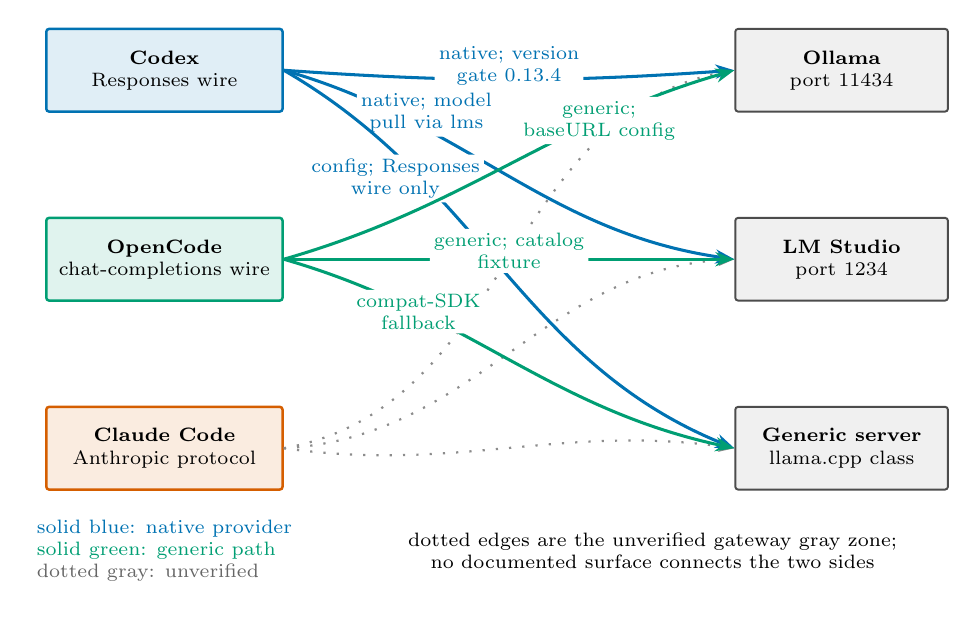
\begin{tikzpicture}[font=\scriptsize,
      chip/.style={align=center, inner sep=1.5pt, fill=white, rounded corners=1pt}]
      \node[ag=nativecol] (cx) at (0, 2.4) {\textbf{Codex}\\ Responses wire};
      \node[ag=genericcol] (oc) at (0, 0.0) {\textbf{OpenCode}\\ chat-completions wire};
      \node[ag=unattcol] (cc) at (0,-2.4) {\textbf{Claude Code}\\ Anthropic protocol};
      \node[sv] (ol) at (8.6, 2.4) {\textbf{Ollama}\\ port 11434};
      \node[sv] (lm) at (8.6, 0.0) {\textbf{LM Studio}\\ port 1234};
      \node[sv] (gn) at (8.6,-2.4) {\textbf{Generic server}\\ llama.cpp class};
      \draw[unv] (cc.east) to[out=10, in=190] (ol.west);
      \draw[unv] (cc.east) to[out=3, in=183] (lm.west);
      \draw[unv] (cc.east) to[out=-8, in=172] (gn.west);
      \draw[nat] (cx.east) to[out=-4, in=184]
        node[chip, pos=0.5, yshift=5pt, text=nativecol] {native; version\\ gate 0.13.4} (ol.west);
      \draw[nat] (cx.east) to[out=-16, in=172]
        node[chip, pos=0.30, yshift=6pt, text=nativecol] {native; model\\ pull via lms} (lm.west);
      \draw[nat] (cx.east) to[out=-30, in=158]
        node[chip, pos=0.22, yshift=-9pt, text=nativecol] {config; Responses\\ wire only} (gn.west);
      \draw[gen] (oc.east) to[out=16, in=196]
        node[chip, pos=0.72, text=genericcol] {generic;\\ baseURL config} (ol.west);
      \draw[gen] (oc.east) to[out=0, in=180]
        node[chip, pos=0.5, yshift=3pt, text=genericcol] {generic; catalog\\ fixture} (lm.west);
      \draw[gen] (oc.east) to[out=-16, in=168]
        node[chip, pos=0.28, text=genericcol] {compat-SDK\\ fallback} (gn.west);
      \node[align=left, font=\scriptsize] at (0,-3.7)
        {\textcolor{nativecol}{solid blue: native provider}\\
         \textcolor{genericcol}{solid green: generic path}\\
         \textcolor{black!60}{dotted gray: unverified}};
      \node[align=center, font=\scriptsize, text width=6.4cm] at (6.2,-3.7)
        {dotted edges are the unverified gateway gray zone;\\ no documented surface connects the two sides};
    \end{tikzpicture}
  \note{Same matrix as the report table, drawn as a graph. Edge styles
  encode tier plus certainty; the labels repeat both, so the figure reads
  in grayscale too.}
\end{frame}

\section{Synthesis}

\begin{frame}{Part II is Part I under stress}
  \begin{columns}[T]
    \column{0.48\textwidth}
      \textbf{What converges}
      \begin{itemize}
        \item the abstract prompt, sample, execute, continue loop
        \item structured edit protocols over free-form shell edits
        \item extension vocabulary: hooks, skills, agents, MCP
        \item dangerous defaults gated behind enterprise layers
      \end{itemize}
    \column{0.48\textwidth}
      \textbf{What genuinely diverges}
      \begin{itemize}
        \item control flow: state machine vs.\ persistence loop vs.\
          closed loop
        \item tool registration: conditional vs.\ fixed vs.\ partly
          documented
        \item safety substrate: prevent vs.\ recover vs.\ layered
        \item compaction trigger: fraction vs.\ reserved buffer vs.\
          undisclosed
        \item state: JSONL-first vs.\ SQL-event-first vs.\ undisclosed
      \end{itemize}
  \end{columns}
  \note{Part I's answer: the naming layer converges while the substrate
  diverges on trust boundary placement, state durability, and interface
  unification.}
\end{frame}

\begin{frame}{The directional claim}
  \textbf{Compatibility with open models is decided by the wire protocol
  an agent commits to, and Part I's architecture predicts each bet.}

  \vspace{0.6em}
  \begin{itemize}
    \item \textcolor{nativecol}{Codex} pinned to Responses and built
    native plumbing for two local servers, accepting the patch-tool loss.
    \item \textcolor{genericcol}{OpenCode} pinned to nothing and accepts
    anything chat-completions-shaped, accepting misbehaving defaults.
    \item \textcolor{unattcol}{Claude Code} commits to Anthropic's stack
    and leaves the rest to an unattested gateway.
  \end{itemize}

  \vspace{0.6em}
  Each bet has a matching price, paid in a different currency. The
  patch-tool thread runs through both parts: one model-ID gate, three
  downstream consequences.
  \note{Every bullet traces to the agent findings frames; the
  cross-reading ties Part II to the configuration dimension of Part I.}
\end{frame}

\begin{frame}{Limitations}
  \begin{itemize}
    \item \textbf{Nothing was executed.} No server started, no model
    called; every statement is a code path or a documentation contract.
    \item \textbf{Version bounds.} Three pinned commits and docs
    snapshots of 2026-08-20; nothing generalizes to newer releases; the
    \occ{} pin is a \texttt{dev} branch.
    \item \textbf{Closed core.} \ccc{}'s loop, tool registry, compaction
    numbers, session storage, enforcement internals, and gateway wire
    shape remain open~\citep{claudeCodePluginSurface,claudeCodeModelDocs}.
    \item \textbf{Provenance hedges.} The Ollama post is from 2024; LM
    Studio live docs were unreachable, so we cite the docs-repo mirror;
    Codex fallback metadata (including the 272k claim) and OpenCode's
    compaction paths are reported with explicit uncertainty; vLLM absent.
  \end{itemize}
\end{frame}

\begin{frame}{Takeaways}
  \begin{enumerate}
    \item The abstraction is settled; the engineering culture is not.
    Choose by trust boundary placement, state durability, and interface
    unification.
    \item Recoverability is a safety mechanism: per-step snapshots with
    revert allow a permissive default policy.
    \item The cheapest open-model entry point today is
    \textcolor{genericcol}{OpenCode's} generic path: configure a base URL
    and fill in limits, or accept wrong accounting.
    \item The most integrated entry point is \textcolor{nativecol}{Codex},
    at the price of the Responses bet on server-side adoption.
    \item For \textcolor{unattcol}{Claude Code}, open-model support
    currently lives in the community router, not in the product.
  \end{enumerate}

  \vspace{0.4em}
  Every claim is bounded to the pinned commits (\texttt{af70018},
  \texttt{d545d8f}, \texttt{c3d2e35}) and the snapshots of 2026-08-20.
  \note{End the talk on the two readings: architecture cultures, and the
  wire protocol as the compatibility variable.}
\end{frame}

\begin{frame}[allowframebreaks]{References}
  \footnotesize
  \bibliographystyle{plainnat}
  \bibliography{refs}
  \note{All entries carry pinned commits or snapshot provenance.}
\end{frame}

\appendix

\begin{frame}{Backup: evidence ledger}
  \begin{itemize}
    \item 44 registry entries: 20 codebase, 17 docs, 3 preprints, 4
      blog-tier context (teardowns and one community router); 47 notes
      (44 source notes plus the combined and per-part syntheses).
    \item 12 Part I claims advanced to ANALYZED with supported evidential
      status (\texttt{CLM-E1-1a} to \texttt{CLM-E4-3a});
      \texttt{CLM-E2-1b} corrected a registration count from 33 to 32
      during review.
    \item Pinned checkouts: \codex{} \texttt{af70018} (main), \occ{}
      \texttt{d545d8f} (dev), \ccc{} surface \texttt{c3d2e35} (main),
      pinned 2026-08-19 and re-pinned 2026-08-20.
  \end{itemize}
\end{frame}

\begin{frame}{Backup: teardown claims held at context tier}
  \begin{itemize}
    \item Intercepted-log teardown: system-prompt and tool-token sizes,
      small-model routing (unverified)~\citep{minusXClaudeCodeTeardown}.
    \item Binary analysis: 243 feature flags, 1{,}163 telemetry events,
      49 built-in tools at one version (unverified)~\citep{tenguDecoded}.
    \item Trace-based breakdown: CLAUDE.md delivery shape, cross-verified
      against official memory docs; only that overlap is reinforced~\citep{agiflowClaudeCodeInternals,claudeCodeDocsMemory}.
  \end{itemize}
\end{frame}

\begin{frame}{Backup: degradation constants}
  \textbf{Codex fallback-metadata gaps}~\citep{codexRepo}:
  \begin{itemize}
    \item \path{apply_patch} is not registered under fallback metadata.
    \item The 272{,}000-token context claim is unverified for the
    catalog-miss path.
  \end{itemize}
  \textbf{OpenCode defaults}~\citep{opencodeRepo}:
  \begin{itemize}
    \item \path{context} $=0$ disables auto-compaction entirely.
    \item \path{output} $=0$ becomes \path{OUTPUT_TOKEN_MAX}$=32{,}000$.
    \item token estimate: \path{characters / 4}.
  \end{itemize}
\end{frame}

\begin{frame}{Backup: gray-zone conditions}
  \begin{itemize}
    \item \path{ANTHROPIC_BASE_URL}: documented, wire shape unattested.
    \item \path{ANTHROPIC_CUSTOM_MODEL_OPTION}: ``you can use any string
    your API endpoint accepts''~\citep{claudeCodeModelDocs}.
    \item \path{CLAUDE_CODE_MAX_CONTEXT_TOKENS}: applies only when the
    model name does not start with \texttt{claude-}, is not a
    \texttt{[1m]} variant, and does not resolve to a Claude
    model~\citep{claudeCodeModelDocs}.
  \end{itemize}
\end{frame}

\begin{frame}{Backup: open gaps (evidence, not absence)}
  \begin{enumerate}
    \item \ccc{}: numeric compaction thresholds; turn-loop
      implementation; full tool registry; provider plumbing; sandbox
      enforcement internals; gateway wire shape.
    \item \occ{}: permission merge precedence; runtime enforcement of
      several schema defaults; compaction path selection (v1 vs.\ v2).
    \item \codex{}: remote model-catalog contents (server-side state);
      catalog-refresh decoding against plain \path{/v1/models} listings.
    \item Server-side acceptance of agent request fields (tools JSON,
      parallel calls, reasoning fields) is uncheckable from both sides.
  \end{enumerate}
\end{frame}

\end{document}
